\documentclass[../Main/Main.tex]{subfiles}
\begin{document}
El modelo general presentado en este trabajo, aunque pesado en notación y relativamente abstracto, resultó ser muy efectivo al llevarlo a la práctica. A lo largo de este capítulo, se hará una exploración intuitiva y visual de sus capacidades. Se remarca que todas las gráficas presentadas, se generaron con el mismo paquete \verb|bpwpm| que realiza la estimación de los parámetros $\bm{\beta}$. Pues, los mismos objetos que las funciones devuelven, pueden ser utilizados para hacer gráficas que evalúan el modelo y reflejen la intuición subyacente. 

Para mostrar los resultados y las capacidades del modelo se presentan seis ejemplos breves. Los primeros cinco, corresponden a bases de datos simuladas en dos dimensiones, es decir, se tienen dos covariables ($\xni\in\mathbb{R}^2 \;\forall i$),  con diferentes patrones para las respuestas $\ysn$ con fronteras tanto lineales como no lineales. El objetivo, es poder visualizar lo flexibles que son las fronteras de clasificación: la parte no lineal del modelo. Asimismo, al trabajar con bases de datos donde $\mathcal{X}^2\subseteq\mathbb{R}^2$, se puede visualizar la función $\eta(\xsn)$ en tres dimensiones. El último ejemplo corresponde a una base de datos médicos reales donde cada observación representa un tumor que pueden o no ser cancerígeno, las covariables representan ciertas características sobre este. Al aumentar la dimensionalidad, el modelo ya no es representable visualmente pero se siguen obteniendo buenos resultados.

A todos los modelos presentados a lo largo de este capítulo se les realizó un análisis de convergencia mirando las medias ergódicas de las cadenas. Sin embargo, únicamente se estudia a detalle para el ejemplo 2 de forma que no se saturara más la presentación. %... Aguas con esta referencia

\section{Evaluación del modelo}
Antes de poder presentar los ejemplos, se definen las dos métricas que se usarán para probar la efectividad (y precisión) de los modelos. Al trabajar con modelos de clasificación binaria, una forma intuitiva de medir su efectividad es a través de un simple conteo de \textit{errores y aciertos}. Este conteo, se presenta en una \textit{matriz de confusión} que desglosa la clasificación en sus respectivas categorías binarias. Asimismo, se presenta la función \textit{log-loss} ($ll$) que no solo pondera la clasificación sino la \textit{precisión} de esta, medida a través de las probabilidades ajustadas $\hat{p}_i$ que se le asigna a cada observación $i$.

Las matrices de confusión (tabla \ref{tab:MatrizConfusion}), son un método descriptivo con base en las tablas de contingencia que calcula la frecuencia de los aciertos y errores separando por grupos. Donde $\hat{y}$ es la variable predicha de la respuesta $y$ y $\#$ el símbolo que denota \textit{número de}. Asimismo, se define la precisión del modelo como:
$$ \text{precisión} = \dfrac{\text{Número de clasificaciones correctas}}{\text{Número total de observaciones}}$$

\begin{table}[H]
\centering
$\begin{array}{c|c|c|l}
~ & \hat{y} = 0 & \hat{y} = 1 & ~ \\[4pt]
\hline
y = 0 & \#0\text{'s } \checkmark & \;\# 0\text{'s clasificados como }1 & \#\text{ de observaciones 0} \\[4pt]
\cdashline{1-4}
y = 1 & \;\# 1\text{'s clasificados como }0 & \# 1\text{'s } \checkmark & \#\text{ de observaciones 1} \\[4pt]
\hline
~ & \# \text{ de 0's estimados} & \# \text{ de 1's estimados } &  \text{Total de obs. = } n
\end{array}$
\caption{La matriz de confusión}
\label{tab:MatrizConfusion}
\end{table}

Sin embargo, la matriz de confusión resulta deficiente para comprar modelos completamente diferentes que resulten en exactamente la misma clasificación, por ello, se define una métrica más formal. Sea $\ysn = (y_1,\ldots,y_n)^t$ el vector de respuestas observadas y \linebreak $\hat{\psn} = (\hat{p_1},\ldots,\hat{p_n})^t$ el vector de probabilidades ajustadas, donde: $$\hat{p}_i = \hat{P}_{\text{modelo}}(y_i = 1\,|\,\xsn_i)$$ es la probabilidad estimada por el modelo de que la observación $y_i$ sea igual a uno. Con lo anterior, se define un vector de respuestas ajustadas $\hat{\ysn} = (\hat{y}_1,\ldots,\hat{y}_n)^t$, haciendo la predicción en el corte $\hat{y_i} = 1 \iff \hat{p}_i > 0.5\,$.\footnote{Este corte, es resultado de la simetría en cero de la función de acumulación normal estándar $\Phi$, derivado de la ecuación \eqref{ec:RegMedia}.}
\begin{definition}
La función \textit{log-loss} $ll:\left\{0,1\right\}^n\times[0,1]^n\rightarrow \mathbb{R}^+$:
\begin{align}
	ll(\ysn,\hat{\psn}) = -\sum_{i = 1}^n[ y_i \ln(\hat{p_i}) + (1-y_i)\ln(1-\hat{p_i})]. \label{ec:LogLoss}
\end{align}
\end{definition}
La ventaja de usar la función $ll$, es que resulta en una métrica que, no sólo mide que tan buena es la clasificación binaria, sino, que toma en cuenta la precisión de la predicción. Idealmente $ll = 0$ si se da una clasificación perfecta y conforme tome valores más positivos, el modelo realiza una peor predicción. Esto se debe a que la función es convexa y se penaliza cuando las probabilidades ajustadas están muy lejos de la real. Asimismo, si la predicción fue incorrecta pero la probabilidad fue cercana a $0.5$ no se penaliza tanto.  En la práctica y bajo un enfoque frecuentista, la función $ll$ puede ser vista como una función de costos y más recientemente se ha utilizado para para entrenar y comparar modelos de clasificación como lo son las redes neuronales \autocite{nielsen2015neural}.

\section{Ejemplo 1 - las capacidades del modelo \texttt{bpwpm} } \label{sec:T1}
El primer ejemplo que se analizará, busca ejemplificar los componentes del modelo en general y sus capacidades. Para ello, se simularon un total de $n = 350$ observaciones separadas en dos grupos, cada uno con tamaños $n_{0} = 200$ y  $n_{1} = 150$ respectivamente ($n = n_0 + n_1$). Los datos se muestrearon de dos distribuciones normales bivariadas:
\begin{align*}
\underset{i = 1,\ldots,200}{\text{Grupo 0: }} \quad 
&\xsn_i \sim \normbivar{2}{2}{0.25}{0.35}{1}{0} \\[6pt]
\underset{i = 201,\ldots,350}{\text{Grupo 1: }} \quad 
&\xsn_i \sim \normbivar{4}{4}{1}{-0.24}{0.64}{1} 
\end{align*}
Las medias $\bm{\mu}_j \; j = \left\{0,1\right\}$ se toman relativamente alejadas y las covarianzas corresponden a las correlaciones $\rho_0 = 0.7$ y $\rho_1 = 0.3$ respectivamente. Estos parámetros de simulación se escogen a través de un proceso empírico resultando en una estructura simple donde los grupos están claramente separados y hay poco traslape. Asimismo, el espacio de covariables queda definido: $\mathcal{X}^2 \approx [0.3,7.5]\times[-0.5,5.9]$. Se codifica el grupo 0, $(y = 0)$, de color rojo y el grupo 1, $(y = 1)$, de color azul.\footnote{Se recomienda visualizar la versión digital de este trabajo donde se aprecian con más claridad los colores. Disponible en \url{https://github.com/PaoloLuciano/Tesis-Latex/}} La base de datos final se presenta en la figura \ref{fig:Test1Plot}.
\begin{figure}[h]
  \centering
      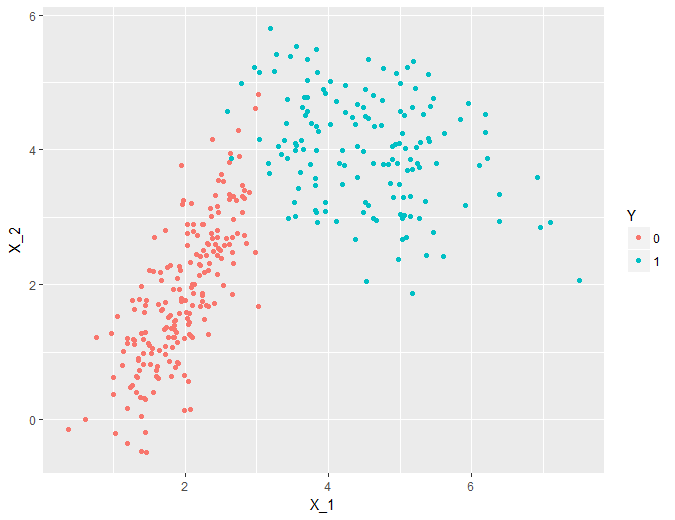
\includegraphics[width = .8\textwidth]{Tests/Test1/GroupPlot}
  \caption{Ejemplo 1 - datos normales bivariados}
 \label{fig:Test1Plot}
\end{figure}

\subsubsection*{Tres realizaciones del modelo}
El objetivo principal de esta simple base de datos es ejemplificar el tipo de fronteras alcanzables por $\eta$, mostrando una clara separación entre los dos grupos sin sobre-ajustar, para ello, se corren tres realizaciones del modelo. Para la primera se escoge el modelo más sencillo, una frontera lineal con un solo nodo (M = 2, J = 2 y K = 1). La segunda realización, consta de parábolas continuas más no suaves sobre cuatro nodos (M = 3, J = 5 y K = 1). Finalmente la tercera realización consta de splines cúbicos en 3 nodos (M = 4, J = 3 y K = 3),\footnote{Polinomios por partes cúbicos suaves hasta la segunda derivada.} en la tabla \ref{tab:Ejemplo1Modelos} se resume lo anterior.\footnote{Se recuerda que $M-1$ corresponde al grado de los polinomios, $J-1$ es el número de nodos, $K$ el parámetro que controla la suavidad, $\N = JM - K(J-1) - 1$ el número de funciones base (por expansión de cada covariable) y $\lambda = 1 + d*\N$ el número total de parámetros.}
\begin{table}[H]
\centering
\begin{tabular}{l|lll}
\hline
Parámetro & Realización 1 & Realización 2 & Realización 3 \\ \hline\hline
$M$       & 2        & 3        & 4        \\ \hline
$J$       & 2        & 5        & 3        \\ \hline
$K$       & 1        & 1        & 3        \\ \hline\hline
$\N$      & 2        & 10       & 5        \\ \hline
$\lambda$ & 5        & 21       & 11       \\ \hline
\end{tabular}
\caption{Ejemplo 1 - tres realizaciones del modelo}
\label{tab:Ejemplo1Modelos}
\end{table}
Para las tres realizaciones se simularon $\nsim = \num{15000}$ valores de $\betabf$ y se opta por no usar periodo de \textit{burn-in} ni suavizamiento para las cadenas, es decir: $k^* = 0$ y $\kthin = 0$, esto para hacer a las cadenas más comparables entre si. La única modificación que se realiza entre las tres realizaciones es que, para la tercera, se estandarizan las covariables.\footnote{Se resta la media y se divide entre la desviación estándar muestral de cada covariable.} Al usar polinomios de orden mayor, en este caso polinomios de tercer grado, el algoritmo puede caer en problemas numéricos pues $\hat{\eta}$ puede crecer muy rápido fuera de $\mathcal{X}^d$; se expande sobre este tema en el capitulo \ref{cap:Conclusiones}. 

En las figuras \ref{fig:T1M1}, \ref{fig:T1M2} y \ref{fig:T1M3} se presentan imágenes que ejemplifican las tres realizaciones del modelo respectivamente. En las imágenes \ref{fig:T1M1Frontera}, \ref{fig:T1M2Frontera} y \ref{fig:T1M3Frontera} se visualizan las diferentes tipos de fronteras que el modelo logra estimar. Con estas fronteras, se nota claramente como es determinante la elección de $\MJK$ en sus formas. El modelo logra estimar tanto fronteras relativamente rígidas (imágen \ref{fig:T1M1Frontera}) como fronteras más suaves en las imágenes subsecuentes \ref{fig:T1M2Frontera} y \ref{fig:T1M3Frontera}. Asimismo, para cada realización, se tiene la representación en 3D de cada función $\hat{\eta}$ que preserva la suavidad (o rugosidad) de sus componentes. Asimismo, rescatando las ideas de los GAM, se puede colapsar cada expansión de polinomios por partes en sus correspondientes funciones $\hat{f}_j$ y visualizarla como la transformación no lineal de cada covariables. Por ejemplo, en la imagen \ref{fig:T1M1F1} se observa que $\hat{f}_1(x_1)$ está compuesta por rectas que se conectan en el nodo, mientras que \ref{fig:T1M3F2} representa $\hat{f}_2(x_2)$, un polinomio cúbico suave hasta la segunda derivada.  

% Realización 1
\begin{figure}[p]
	\centering
	\begin{subfigure}[b]{0.45\textwidth}
    	\includegraphics[width =\textwidth]{Tests/Test1/T1M1Frontera}
		\caption{Frontera de predicción}
		\label{fig:T1M1Frontera}
	\end{subfigure}
	\hfill    
    \begin{subfigure}[b]{0.45\textwidth}
        \includegraphics[width=\textwidth]{Tests/Test1/T1M13D}
        \caption{Representación 3D de $\hat{\eta}$}
        \label{fig:T1M13D}
    \end{subfigure}
    \\[3pt]
    \begin{subfigure}[b]{0.45\textwidth}
    	\includegraphics[width =\textwidth]{Tests/Test1/T1M1F1}
		\caption{$\hat{f}_1(x_1)$}
		\label{fig:T1M1F1}
	\end{subfigure}
	\hfill    
    \begin{subfigure}[b]{0.45\textwidth}
        \includegraphics[width=\textwidth]{Tests/Test1/T1M1F2}
        \caption{$\hat{f}_2(x_2)$}
        \label{fig:T1M1F2}
    \end{subfigure}
    \caption{Realización 1 - fronteras lineales con un nodo (M = 2, J = 2 y K = 1)}
    \label{fig:T1M1}
\end{figure}

% Realización 2
\begin{figure}[p]
	\centering
	\begin{subfigure}[b]{0.45\textwidth}
    	\includegraphics[width =\textwidth]{Tests/Test1/T1M2Frontera}
		\caption{Frontera de predicción}
		\label{fig:T1M2Frontera}
	\end{subfigure}
	\hfill    
    \begin{subfigure}[b]{0.45\textwidth}
        \includegraphics[width=\textwidth]{Tests/Test1/T1M23D}
        \caption{Representación 3D de $\hat{\eta}$}
        \label{fig:T1M23D}
    \end{subfigure}
    \\[3pt]
    \begin{subfigure}[b]{0.45\textwidth}
    	\includegraphics[width =\textwidth]{Tests/Test1/T1M2F1}
		\caption{$\hat{f}_1(x_1)$}
		\label{fig:T1M2F1}
	\end{subfigure}
	\hfill    
    \begin{subfigure}[b]{0.45\textwidth}
        \includegraphics[width=\textwidth]{Tests/Test1/T1M2F2}
        \caption{$\hat{f}_2(x_2)$}
        \label{fig:T1M2F2}
    \end{subfigure}
    \caption{Realización 2 - parábolas continuas mas no suaves (M = 3, J = 5 y K = 1)}
    \label{fig:T1M2}
\end{figure}

% Realización 3
\begin{figure}[p]
	\centering
	\begin{subfigure}[b]{0.45\textwidth}
    	\includegraphics[width =\textwidth]{Tests/Test1/T1M3Frontera}
		\caption{Frontera de predicción}
		\label{fig:T1M3Frontera}
	\end{subfigure}
	\hfill    
    \begin{subfigure}[b]{0.45\textwidth}
        \includegraphics[width=\textwidth]{Tests/Test1/T1M33D}
        \caption{Representación 3D de $\hat{\eta}$}
        \label{fig:T1M33D}
    \end{subfigure}
    \\[3pt]
    \begin{subfigure}[b]{0.45\textwidth}
    	\includegraphics[width =\textwidth]{Tests/Test1/T1M3F1}
		\caption{$\hat{f}_1(x_1)$}
		\label{fig:T1M3F1}
	\end{subfigure}
	\hfill    
    \begin{subfigure}[b]{0.45\textwidth}
        \includegraphics[width=\textwidth]{Tests/Test1/T1M3F2}
        \caption{$\hat{f}_2(x_2)$}
        \label{fig:T1M3F2}
    \end{subfigure}
    \caption{Realización 3 - \textit{splines} cúbicos (M = 4, J = 3 y K = 3)}
    \label{fig:T1M3}
\end{figure}

\begin{table}[h]
\begin{subtable}[t]{0.45\textwidth}
	\centering
	$\matconf{198}{2}{200}{2}{148}{150}{200}{150}{350}$
	\caption{Matriz de confusión para todas las realizaciones}
	\label{tab:T1MatConf}
\end{subtable}
\hfill
\begin{subtable}[t]{0.45\textwidth}
	\centering
	$\begin{array}{c|c}
		\text{Realización} & ll \\ \hline\hline
		1 & 0.04088 \\
		2 & 0.03464 \\
		3 & 0.03498
	\end{array}$
	\caption{\textit{log-loss}}
	\label{tab:T1ll}
\end{subtable}
\caption{Ejemplo 1 - resultados}
\label{tab:T1Resultados}
\end{table}
Al estar tratando con una base de datos tan sencilla, no es el enfoque comparar los resultados de estas realizaciones entre si pues las tres logran exactamente la misma clasificación desglosada en la tabla \ref{tab:T1MatConf}. Al compartir la matriz de confusión, por ende, las realizaciones también comparten una precisión de $98.9\%$. De la matriz y las imágenes, se observa que se clasifican de forma incorrecta solo cuatro observaciones. Sería inverosímil tratar de alcanzar una precisión del $100\%$ pues implicaría sobre-ajsutar el modelo. Para estas cuatro observaciones incorrectamente clasificadas, no se tiene la suficiente evidencia como para clasificarlas en su categoría contraría. Sin embargo, los modelos se pueden comparar más a fondo por medio de la métrica $ll$ presentada en la tabla \ref{tab:T1ll}. Aunque muy similares, la definición de la métrica indica que la realización dos es la mejor por un pequeño margen pues es la más cercana a cero. Claro está, bajo esta comparación no se toma en cuenta el número de parámetros, es decir, la complejidad del modelo en si.

Dado que este es un ejemplo introductorio la estimación de los parámetros, se realizó \textit{dentro de la muestra} (\textit{in-sample}) esto quiere decir, que el modelo se entrena con las mismas observaciones contra las que se busca predecir.\footnote{El efecto que esto puede tener es que se sobre-ajuste o se hagan predicciones demasiado acertadas. De cualquier forma el paquete incluye funcionalidad como para permitir un entrenamiento previo y una predicción \textit{fuera de muestra} (\textit{out-of-sample)}.} Cabe mencionar que para esta sencilla base de datos en particular, usar un modelo complejo como el \textit{bpwpm} no es del todo necesario pues la base podría ser clasificada con la misma precisión por un modelo que use un predictor lineal en covariables. Sin embargo, se usa la base de datos para ejemplificar los tipos de fronteras flexibles. Asimismo, presentar las formas funcionales que toman las funciones $f_j$ tampoco aportaría mucho pues están compuestas de muchos términos aditivos que no vale la pena desglosar. 

\section{Ejemplo 2 - comparación contra un probit lineal} \label{sec:T2}
Aprovechando la familiaridad de la base de datos anterior, se decide modificarala para que existan dos regiones de clasificación separadas. Se tomaron trece puntos, más allá de $x_1 \approx 5.5$ y se voltea su clasificación. En la imagen \ref{fig:T2Datos} se presenta esta base de datos modificada. 

Con afán de comparar las predicciones del modelo \textit{bpwpm} presentado en este trabajo contra uno más convencional, primeramente se corre un modelo probit lineal en covariables. Es decir, se estiman los parámetros $\bm{\beta} = (\beta_0,\beta_1,\beta_2)^t$ del modelo:\footnote{La estimación se realiza bajo el paradigma frecuentista usando el método de mínimos cuadrados a través de la función \texttt{glm(..., family = binomial(link = 'probit'))} en \texttt{R}.} 
\begin{align}
	p_i & = P(y_i = 1) =\E[y|\xni] = \Phi(\eta(\xni))  \quad \Rightarrow  			\nonumber \\
	\eta(\xni) = \Phi^{-1}(p_i) &= \beta_0 + \beta_1x_{i,1} + \beta_2x_{i,2} 
	\qquad 	\forall i =1,\ldots,n \label{ec:T2GLM}
\end{align}
De donde se obtienen los resultados presentados en la tabla \ref{tab:T2GLMRes} y la figura \ref{fig:T2GLM}. De la imagen anterior, todo lo que quede por arriba de recta será clasificado como uno y todo lo que quede por debajo como cero.
\begin{figure}[h]
	\centering
   	\includegraphics[width =0.95\textwidth]{Tests/Test2/T2GLM}
	\caption{Frontera de predicción para modelo probit lineal en covariables}
	\label{fig:T2GLM}
\end{figure}

\begin{table}[h]
	\begin{subtable}[t]{0.45\textwidth}
		\centering
		$\begin{array}{c|c}
		\text{Parámetro} &\text{Estimado} \\
		\hline\hline
		\hat{\beta_0} & -4.67\\
		\hat{\beta_1} & 0.45 \\
		\hat{\beta_2} & 0.91 \\
		\end{array}$
	\end{subtable}
	\hfill
	\begin{subtable}[t]{0.45\textwidth}
		\centering
		$\resultados{\text{No aplica}}{90}{0.28072}$
	\end{subtable}
	\vskip\baselineskip
	\begin{subtable}[t]{\textwidth}
		\centering
		$\matconf{194}{19}{213}{16}{121}{137}{210}{140}{350}$
	\end{subtable}		
	\caption{Ejemplo 2 - resultados para modelo probit lineal}
	\label{tab:T2GLMRes}
\end{table}

Por ende, el modelo resultante es:
\begin{align}
 \Phi^{-1}(\hat{p}_i) &= \hat{\eta}(\xsn) = -4.67 + 0.45x_{i,1} + 0.91x_{i,2}, \label{ec:T2GLMEst}
\end{align}
de donde se puede obtener explicitamente la ecuación de la frontera de predicción igualando \eqref{ec:T2GLMEst} a 0.5, es decir:
\begin{align}
	\Phi(\hat{\eta}(\xni)) &\equiv 0.5 \qquad \iff \nonumber \\
	\hat{\eta}(\xni) &= 0 \;\;\qquad \iff  \nonumber \\
	0.45x_{i,1} + 0.91x_{i,2} &= 4.67  \label{ec:T2RectaGLM}
\end{align}

Para contrastar, ahora se corre el modelo \textit{bpwpm} especificando $M = 3, J = 3$ y $K =2$ (resumen en la tabla \ref{tab:T2}). Para este ejemplo, se opta por analizar a fondo todos los componentes y hacer un análisis más detallado de su convergencia, por lo tanto, se presentan los resultados de los estimadores en la tabla \ref{tab:T2Res} e imágenes generadas en la figura \ref{fig:T2Plots}.
\begin{table}[h]
$$\paramsmod{3}{3}{2}{4}{9}{350}{\num{10000}}{\num{7500}}{0}$$
\caption{Ejemplo 2 - regiones disjuntas de clasifcación}
\label{tab:T2}
\end{table}

Juntando todo, el modelo final como forma funcional a:
\begin{align}
	\Phi^{-1}(\hat{p}_i) = &\; \hat{\eta}(\xsn) = \hat{f}_0 + \hat{f}_1(x_{i,1}) +  \hat{f}_2(x_{i,2}) \label{ec:T2}\\[5pt]	
	= & \overbrace{\hat{\beta}_0}^{\hat{f}_0} \nonumber \\ 
	+ & \overbrace{\hat{\beta}_1x_{i,1} + \hat{\beta}_2x_{i,1}^2 
+ \hat{\beta}_3(x_{i,1} - \hat{\t}_{1,1})_+^2 + \hat{\beta}_4(x_{i,1} - \hat{\t}_{1,2})_+^2}^{\hat{f}_1(x_{i,1})} \nonumber \\
	+ & \overbrace{\hat{\beta}_5x_{i,2} + \hat{\beta}_6x_{i,2}^2 
+ \hat{\beta}_7(x_{i,2} - \hat{\t}_{2,1})_+^2 + \hat{\beta}_8(x_{i,2} - \hat{\t}_{2,2})_+^2}^{\hat{f}_2(x_{i,2})}\quad, \nonumber
\end{align}
la cual queda perfectamente definida si se sustituyen los valores de $\betabf$ y nodos contenidos en $\P$ presentados en la tabla \ref{tab:T2Res}. La ecuación \eqref{ec:T2} permite observar la expansión en bases final de $\eta(\cdot)$ para esta realización y elección de parámetros. Asimismo, en esta expansión se observa su forma aditiva y el desglose de las funciones $\hat{f}_j$. Es necesario remarcar que la transformación que realizan las funciones no lineales $f_j$, se observa contrastando las imágenes \ref{fig:T2Datos} y \ref{fig:T2FSpace}. Es decir, el espacio inicial de covariables $\mathcal{X}^2$ (imagen \ref{fig:T2Datos}) tiene una forma que no puede ser separable por una frontera lineal. Sin embargo al llevar a cabo la transformación no lineal de esta base (imagen \ref{fig:T2Datos}), se deriva en un espacio $\widetilde{\Psi}(\mathcal{X})^{9}$ que si puede ser separable por una recta. En consecuencia, la frontera de clasificación es disjunta, pues el modelo identifica dos regiones donde los datos deben ser clasificados como cero (imágenes \ref{fig:T2Frontera} y \ref{fig:T23D}). Una vez más, se tienen esos pocos puntos que no quedan bien clasificados, incluyendo uno nuevo cerca de las coordenadas cartesianas $(5.8, 2.3)$. Para esta base de datos en particular, se debe usar un nodo adicional cerca de la segunda región, ya que la curvatura, deriva de él. Asimismo, la suavidad de las funciones $\hat{f}$ deriva de la elección de $K$.
%Como se observa en la imagen \ref{fig:T23D}, la \textit{sabana} que antes era creciente a medida que $x_1$ crecía, ahora se vuelve a curvar, volviéndose negativa otra vez y clasificando bien la segunda sección roja.

Contrastando los resultados del modelo probit lineal (tabla \ref{tab:T2GLMRes}) contra el modelo \textit{bpwpm} (tabla \ref{tab:T2Res}), se observa que se tiene una mejora en precisión sustancial pues se enfatiza que la flexibilidad en la frontera viene derivada del número relativamente grande de parámetros. Uno de los beneficios es que para el modelo probit lineal, esta frontera se puede derivar de forma explicita la ecuación \eqref{ec:T2RectaGLM}, mientras que para el modelo \textit{bpwpm} implicaría resolver numéricamente la ecuación derivada  de la expresión no lineal \eqref{ec:T2}. Asimismo, al compara la métrica \textit{log-loss}, se observa que se tiene una mejora importante. En cuanto a tiempo de estimación computacional, no se tiene una diferencia significativa entre los dos modelos. 

\begin{table}[ph]
	\begin{subtable}[t]{0.45\textwidth}
		\centering
		$\resultados{\text{Media posterior}}{98.6}{0.04505}$
	\end{subtable}
	\hfill
	\begin{subtable}[t]{0.45\textwidth}
		\centering
		$\matconf{210}{2}{200}{2}{135}{137}{212}{138}{350}$
	\end{subtable}
	\vskip\baselineskip
	\begin{subtable}[t]{0.45\textwidth}	
		\centering
		\renewcommand*{\arraystretch}{1.4}
		$\begin{array}{c|cl}
		\bm{\beta} & \text{Valor} & ~ \\
		\hline\hline
		\hat{\beta_0} & -2.03 &  \rdelim\}{1}{0pt}[$\hat{f}_0$]\\
		\hat{\beta_1} & -1.74 &  \rdelim\}{4}{0pt}[$\hat{f}_1(x_{i,1})$]\\
		\hat{\beta_2} & 0.90  & ~ \\
		\hat{\beta_3} & -0.07 & ~ \\
		\hat{\beta_4} & -3.68 & ~ \\
		\hat{\beta_5} & -1.01 &  \rdelim\}{4}{0pt}[$\hat{f}_1(x_{i,1})$]\\
		\hat{\beta_6} & 0.13 & ~ \\
		\hat{\beta_7} & 0.31 & ~ \\
		\hat{\beta_8} & -0.25 & ~ 
		\end{array}$
	\end{subtable}
	\hfill
	\begin{subtable}[t]{0.45\textwidth}
	\centering
	\renewcommand*{\arraystretch}{1.4}
	$\begin{array}{c|cl}
	\mathcal{P} & \text{Valor} & ~ \\
	\hline\hline
	\hat{\t}_{1,1} & 2.07 & \rdelim\}{4}{0pt}[Nodos]\\
	\hat{\t}_{1,2} & 3.69 & ~ \\
	\hat{\t}_{2,1} & 2.00 & ~ \\
	\hat{\t}_{2,2} & 3.52 & ~ 
	\end{array}$
	\end{subtable}
\caption{Ejemplo 2 - resultados}
\label{tab:T2Res}
\end{table}

\begin{figure}[ph]
        \centering 
        \begin{subfigure}[b]{0.45\linewidth}
		   	\includegraphics[width=\linewidth]{Tests/Test2/T2Datos}
			\caption{Base del ejemplo 1 modificada}
			\label{fig:T2Datos}
        \end{subfigure}
        \hfill
        \begin{subfigure}[b]{0.45\linewidth}  
            \includegraphics[width=\linewidth]{Tests/Test2/T2FSpace}
            \caption{Transformación no lineal}
            \label{fig:T2FSpace}
        \end{subfigure}
		\vskip\baselineskip
        \begin{subfigure}[b]{0.45\linewidth}   
            \includegraphics[width=\linewidth]{Tests/Test2/T2Frontera}
            \caption{Frontera de predicción}
            \label{fig:T2Frontera}
        \end{subfigure}
		\hfill
        \begin{subfigure}[b]{0.45\linewidth}   
            \includegraphics[width=\linewidth]{Tests/Test2/T23D}
            \caption{Representación 3D de $\hat{\eta}$}    
            \label{fig:T23D}
        \end{subfigure}
		\vskip\baselineskip
        \begin{subfigure}[b]{0.45\linewidth}  
            \includegraphics[width=\linewidth]{Tests/Test2/T2F1}
            \caption{$\hat{f}_1(x_1)$}
            \label{fig:T2F1}
        \end{subfigure}
		\hfill
		\begin{subfigure}[b]{0.45\linewidth}   
            \includegraphics[width=\linewidth]{Tests/Test2/T2F2}
            \caption{$\hat{f}_2(x_2)$}    
            \label{fig:T2F2}
        \end{subfigure}    
	\caption{Ejemplo 2 - regiones disjuntas de clasificación ($M = 3$, $J = 3$ y $K = 2$)}
	\label{fig:T2Plots}
\end{figure}

\pagebreak
\subsection{Análisis de convergencia} \label{sec:AnalisisConv}
Para finalizar este ejemplo, se busca realizar un análisis detallado de la convergencia de las cadenas pues es parte fundamental del estudio de un modelo bayesiano. Por lo tanto en la tabla \ref{tab:T2Betas} se presentan resúmenes numéricos de los parámetros $\betabf$ y las cadenas completas en la figura \ref{fig:T2Conv}.\footnote{Tanto las imágenes como los resúmenes, aún no han sido ajustados por el periodo de burn-in, de ahí la disparidad contra las estimaciones puntuales de \ref{tab:T2Res}. Asimismo, para este ejemplo se presenta una visualización animada en formato \texttt{.gif} de como el algoritmo converge conforme avanza el número de iteraciones, consultando \href{https://github.com/PaoloLuciano/Tesis-Latex}{\texttt{https://github.com/PaoloLuciano/Tesis-Latex}}}

Al analizar las gráficas y los resúmenes, se nota como ciertos parámetros como $\hat{\beta}_4$ fluctúan mucho en su estimación en un comienzo, sin embargo de \ref{fig:T2ME} se observa como el modelo converge a la larga. Asimismo, de los histogramas y trazas de las cadenas, se observa que estas tienden a estar bien formadas y presentan vagamente una distribución normal multivariada, estabilizandose conforme el algoritmo de muestreo Gibbs converge al espacio de probabilidad buscado. El periodo de burn-in, se escoge en $k* = 7,500$ pues se busca dar estimaciones puntuales de la media posterior lo más exactas posibles y pareciera que a partir de $k*$ se logra esto pues tanto las cadenas como la media ergódica no fluctúa demasiado. Si únicamente se mostraran los datos de las cadenas recordadas, los histogramas estarían perfectamente formados y tendrían una desviación estándar de aproximadamente uno por construcción.

Para este modelo flexible, aunque los parámetros no estén confundidos, existe la posibilidad de que algunos de ellos convergan a cero pues son innecesarios para la estimación, por ejemplo $\hat{\beta}_3$ y $\hat{\beta}_6$. Para identificar estos parámetros, se pueden aplicar pruebas de hipótesis o procedimientos de selección de variables ya que se cuenta con toda la información que se tendría en un modelo tradicional; sin embargo, se enfatizan los resultados de predicción del modelo completo y no la interpretabilidad de los parámetros individuales.

\vspace{2.5cm}
\begin{table}[ph]
	\begin{subtable}[t]{\textwidth}
		$\begin{array}{l|r:r:r:r:r}
			\text{Métrica}             & \hat{\beta}_0 & \hat{\beta}_1 & \hat{\beta}_2 & \hat{\beta}_3 & \hat{\beta}_4 \\
			\hline\hline
			\text{Mínimo}              & -6.79         & -6.63         & -0.39         & -2.11         & -27.40        \\
			\text{Primer Cuartíl}      & -2.54         & -2.22         & 0.66          & -0.48         & -3.72         \\
			\text{Media}               & -2.03         & -1.73         & 0.90          & -0.07         & -3.68         \\
			\text{Mediana}             & -1.98         & -1.69         & 0.85          & -0.09         & -3.28         \\
			\text{Tercer Cuartíl}      & -1.44         & -1.17         & 1.05          & 0.27          & -2.86         \\
			\text{Máximo}              & 0.85          & 1.56          & 4.21          & 10.38         & -1.07         \\
			\text{Desviación Estandar} & 0.89          & 0.87          & 0.45          & 0.72          & 2.61         
		\end{array}$
	\end{subtable}
		\vskip\baselineskip
	\begin{subtable}[t]{\textwidth}
		$\begin{array}{l|r:r:r:r}
			\text{Métrica}             & \hat{\beta}_5 & \hat{\beta}_6 & \hat{\beta}_7 & \hat{\beta}_8 \\
			\hline\hline
			\text{Mínimo}              & -5.59         & -1.64         & -1.89         & -2.47        \\
			\text{Primer Cuartíl}      & -1.49         & -0.04         & -0.05         & -0.69        \\
			\text{Media}               & -1.00         & 0.13          & 0.31          & -0.21        \\
			\text{Mediana}             & -0.97         & 0.13          & 0.27          & -0.27        \\
			\text{Tercer Cuartíl}      & -0.44         & 0.31          & 0.63          & 0.13         \\
			\text{Máximo}              & 2.44          & 1.47          & 6.67          & 11.0         \\
			\text{Desviación Estandar} & 0.87          & 0.28          & 0.60          & 0.94        
		\end{array}$
	\end{subtable}
	\caption{Ejemplo 2 - resúmenes numéricos para las cadenas de $\betabf$}
	\label{tab:T2Betas}
\end{table}

\begin{figure}[ph]
        \centering 
        \begin{subfigure}[b]{0.45\linewidth}
		   	\includegraphics[width=\linewidth]{Tests/Test2/T2Trazas1}
			\caption{Trazas de $\hat{\beta}_0$ a $\hat{\beta}_4$}
			\label{fig:T2Trazas1}
        \end{subfigure}
        \hfill
        \begin{subfigure}[b]{0.45\linewidth}  
            \includegraphics[width=\linewidth]{Tests/Test2/T2Hist1}
            \caption{Histogramas de $\hat{\beta}_0$ a $\hat{\beta}_4$}
            \label{fig:T2Hist1}
        \end{subfigure}

        \begin{subfigure}[b]{0.45\linewidth}   
            \includegraphics[width=\linewidth]{Tests/Test2/T2Trazas2}
            \caption{Trazas de $\hat{\beta}_5$ a $\hat{\beta}_8$}
            \label{fig:T2Trazas2}
        \end{subfigure}
		\hfill
        \begin{subfigure}[b]{0.45\linewidth}   
            \includegraphics[width=\linewidth]{Tests/Test2/T2Hist2}
            \caption{Histogramas de $\hat{\beta}_5$ a $\hat{\beta}_8$}    
            \label{fig:T2Hist2}
        \end{subfigure}
		\vskip\baselineskip
        \begin{subfigure}[b]{0.45\linewidth}  
            \includegraphics[width=\linewidth]{Tests/Test2/T2ME}
            \caption{Media ergódica}
            \label{fig:T2ME}
        \end{subfigure}
	\caption{Ejemplo 2 - análisis de convergencia}
	\label{fig:T2Conv}
\end{figure}

\pagebreak
\section{Ejemplos 3 a 5 - otros resultados interesantes} \label{sec:T3-5}
Los ejemplos presentados a continuación, son más expositivos que analíticos, es decir, se enfatizan los resultados más que los detalles matemáticos como se hizo en la sección anterior. Estos ejemplos y bases de datos simuladas, buscan sobre todo poner a prueba las capacidades no lineales del modelo y estresar las interacciones entre las dimensiones. Al estar tratando con regiones de clasificación más complejas, la predicción correcta sería imposible para un modelo lineal en covariables.

% Ej 4 - Parábola
\subsection*{Ejemplo 3 - región parabólica}
Para este ejemplo, se generaron $n = 400$ datos en $\mathbb{R}^2$ usando coordenadas polares al tomar ángulos con un rango entre $[-1,1]$. Posteriormente se tomaron diferentes radios para diferenciar cada grupo y finalmente se les sumó ruido blanco a los puntos para que existiera una región de confusión. Las simulación derivó en un patrón de datos cuya frontera es curva, casi parabólica. Dadas las características de los datos, se piensa que usar polinomios por partes parabólicos y suaves ($M = 3$ y $K = 2$) es una buena opción para modelarlos. Los parámetros escogidos para la realización final del modelo, se presentan en la tabla \ref{tab:T3}. Asimismo, los resultados e imágenes se presentan en la tabla \ref{tab:T3Res} y la figura \ref{fig:T3Plots} respectivamente.

\begin{table}[h]
$$\paramsmod{3}{4}{2}{5}{11}{400}{\num{10000}}{\num{2500}}{0}$$
\caption{Ejemplo 3 - región parabólica}
\label{tab:T3}
\end{table}

\begin{table}[h]
\begin{align*}
\resultados{\text{Media posterior}}{99.2}{0.04352}
\qquad\qquad\qquad
\matconf{198}{2}{200}{1}{199}{200}{199}{201}{400}
\end{align*}
\caption{Ejemplo 3 - resultados}
\label{tab:T3Res}
\end{table}

\begin{figure}[p]
        \centering
        \begin{subfigure}[b]{0.45\textwidth}
            \centering
            \includegraphics[width=\textwidth]{Tests/Test3/T3Frontera}
            \caption{Frontera}   
            \label{fig:T3Frontera}
        \end{subfigure}
        \hfill
        \begin{subfigure}[b]{0.45\textwidth}  
            \centering 
            \includegraphics[width=\textwidth]{Tests/Test3/T3FSpace}
            \caption{Transformación no lineal}
            \label{fig:T3FSpace}
        \end{subfigure}
        \vskip\baselineskip
        \begin{subfigure}[b]{0.45\textwidth}   
            \centering 
            \includegraphics[width=\textwidth]{Tests/Test3/T3F1}
            \caption{$\hat{f}_1(x_1)$}
            \label{fig:T3F1}
        \end{subfigure}
		\hfill
        \begin{subfigure}[b]{0.45\textwidth}   
            \centering 
            \includegraphics[width=\textwidth]{Tests/Test3/T3F2}
            \caption{$\hat{f}_2(x_2)$}    
            \label{fig:T3F2}
        \end{subfigure}
		\vskip\baselineskip
        \begin{subfigure}[b]{0.45\textwidth}  
            \centering 
            \includegraphics[width=\textwidth]{Tests/Test3/T33D}
            \caption{Representación 3D de $\hat{\eta}$}
            \label{fig:T33D}
        \end{subfigure}
        \hfill
        \begin{subfigure}[b]{0.45\textwidth}  
            \centering 
            \includegraphics[width=\textwidth]{Tests/Test3/T3ME}
            \caption{Medias ergódicas}
            \label{fig:T3ME}
        \end{subfigure}        
	\caption{Ejemplo 3 - parábolas suaves ($M = 3$, $J = 4$ y $K = 2$)}
	\label{fig:T3Plots}
\end{figure}
Esta es una realización particularmente interesante pues con un total $\lambda = 11$ parámetros se logra una precisión alta además de obtener convergencia relativamente rápido ($\nsim = \num{10000}$ y $k^* = \num{2500}$). Analizando el modelo de forma gráfica, se observa claramente que la segunda transformación $\hat{f}_2(x_2)$ (imagen \ref{fig:T3F2}) captura la parte parabólica. A la vez, la primera transformación $\hat{f}_1(x_1)$ (imagen \ref{fig:T3F1}) le da poco peso a la región donde hay confusión entre los los grupos pero posteriormente crece en donde hay certidumbre.  Asimismo, se presenta el espacio de la transformación no lineal en la imagen \ref{fig:T3FSpace} en donde se observa que el grupo rojo cero, se concentra en la esquina inferior izquierda, representando la posible separación lineal en este espacio transformado. 

\subsection*{Ejemplo 4 - región ovalada}
Para esta base de datos en particular se busca replicar algo similar a la imagen del capítulo introductorio \ref{fig:DiagramaIntro} de la página \pageref{fig:DiagramaIntro}. Se obtuvo una base de datos pequeña del curso en linea de aprendizaje de máquina de \citet{andrew2018ml} que presenta una frontera de clasificación ovalada.\footnote{Este curso, se ofrece de forma gratuita en la plataforma de MOOC's \href{https://www.coursera.org/learn/machine-learning}{Coursera}.} Esta base de datos se usa para entrenar modelos saturados logit con regularización, \citet{hastie2008elements}, logrando predecir fronteras curvas con modelos tradicionalmente lineales al incluir interacciones de orden mayor entre covariables. Por lo tanto, se decidió probarlo también con el modelo presentado para contrastar.

El modelo una vez más, fue ajustado usando parábolas suaves las cuales resultaron ser excelentes herramientas. La parámetros escogidos para la realización final del modelo, se presenta en la tabla \ref{tab:T4} con resultados e imágenes en la tabla \ref{tab:T4Res} y figura \ref{fig:T4Plots} respectivamente.  
\begin{table}[h]
$$\paramsmod{3}{2}{2}{3}{7}{118}{\num{2000}}{500}{0}$$
\caption{Ejemplo 4 - región ovalada}
\label{tab:T4}
\end{table}

\begin{table}[h]
\begin{align*}
\resultados{\text{Media posterior}}{78.8}{0.4714}
\qquad\qquad\qquad
\matconf{48}{12}{60}{13}{45}{58}{61}{57}{118}
\end{align*}
\caption{Ejemplo 4 - resultados}
\label{tab:T4Res}
\end{table}

Para esta realización del modelo, se buscó estresar su flexibilidad al incluir el menor número de términos posibles usando un solo nodo ($\lambda = 7$ y $J = 2$) y cadenas cortas ($\nsim = \num{2000}$). Aunque una precisión de $78.8\%$ no resulte tan atractiva, es la precisión que se presenta en el curso en línea y permanece constante aún si se aumenta $\lambda$. La métrica \textit{ll} mejora (marginalmente) sobre la presentada en el curso ($\approx0.5$), sin embargo, se logra una reducción significativa en el número de parámetros pues el modelo saturado de \citet{andrew2018ml} inicia con 28 parámetros.\footnote{Dada la regularización, muchos de estos parámetros se desvanecían.} Asimismo, como se observa en la figura \ref{fig:T4ME} las cadenas convergen rápidamente. Todo el poder del modelo, recae en la forma funcional de las funciones $\hat{f}_j$ al poder estimar regiones irregularmente curvas, con pocas observaciones y parámetros. 

\begin{figure}[p]
        \centering
        \begin{subfigure}[b]{0.45\textwidth}
            \centering
            \includegraphics[width=\textwidth]{Tests/Test4/T4Frontera}
            \caption{Frontera}   
            \label{fig:T4Frontera}
        \end{subfigure}
        \hfill
        \begin{subfigure}[b]{0.45\textwidth}  
            \centering 
            \includegraphics[width=\textwidth]{Tests/Test4/T4FSpace}
            \caption{Transformación no lineal}
            \label{fig:T4FSpace}
        \end{subfigure}
        \vskip\baselineskip
        \begin{subfigure}[b]{0.45\textwidth}   
            \centering 
            \includegraphics[width=\textwidth]{Tests/Test4/T4F1}
            \caption{$\hat{f}_1(x_1)$}
            \label{fig:T4F1}
        \end{subfigure}
		\hfill
        \begin{subfigure}[b]{0.45\textwidth}   
            \centering 
            \includegraphics[width=\textwidth]{Tests/Test4/T4F2}
            \caption{$\hat{f}_2(x_2)$}    
            \label{fig:T4F2}
        \end{subfigure}
		\vskip\baselineskip
        \begin{subfigure}[b]{0.45\textwidth}  
            \centering 
            \includegraphics[width=\textwidth]{Tests/Test4/T43D}
            \caption{Representación 3D de $\hat{\eta}$}
            \label{fig:T43D}
        \end{subfigure}
		\hfill
		\begin{subfigure}[b]{0.45\textwidth}   
            \centering 
            \includegraphics[width=\textwidth]{Tests/Test4/T4ME}
            \caption{Medias ergódicas}    
            \label{fig:T4ME}
        \end{subfigure}    
	\caption{Ejemplo 4 - parábolas suaves en un nodos ($M = 3$, $J = 2$ y $K = 2$)}
	\label{fig:T4Plots}
\end{figure}

\subsubsection*{Ejemplo 5 - \textit{yin-yang}, limitaciones del modelo}
Para finalizar con las bases de datos simulados, el modelo \textit{bpwpm} se llevó al límite de sus capacidades sobre un patrón de puntos, intuitivo al ojo humano, pero difícil de identificar por un modelo de este tipo. Los datos tratan de simular un \textit{yin-yang} que se puede observar en la figura \ref{fig:YYDatos}. La simple simulación de la base de datos representó un reto donde se conjuntaron varias áreas de la matemática aplicada. En el software \verb|GeoGebra|, se generó el diagrama presentado en la figura \ref{fig:YYGG} que consiste de las siguientes desigualdades cartesianas:
\begin{align*}
	x^2 + y^2 &< 16, \\
	(x+2)^2 + (y-1.5)^2 &< 0.49, \\
	(x-1.5)^2 + (y+2)^2 &< 0.49, \\[4pt]
	x &< \dfrac{y}{(1+y^2).}
\end{align*}

\begin{figure}[h]
        \centering
        \begin{subfigure}[t]{0.45\textwidth}
            \centering
            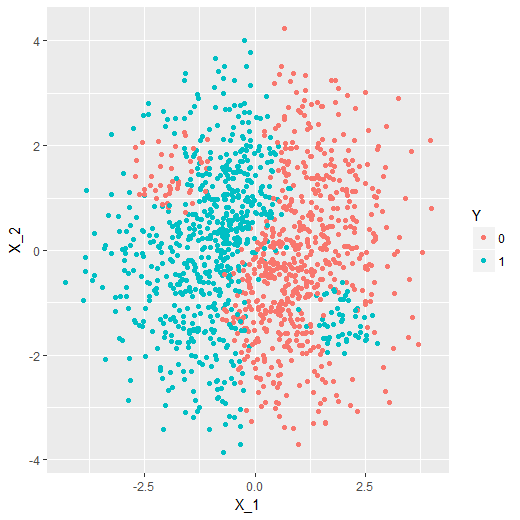
\includegraphics[width=\textwidth]{Tests/Test5/YYDatos}
            \caption{Datos simulados}   
            \label{fig:YYDatos}
        \end{subfigure}
        \hfill
        \begin{subfigure}[t]{0.45\textwidth}  
            \centering 
            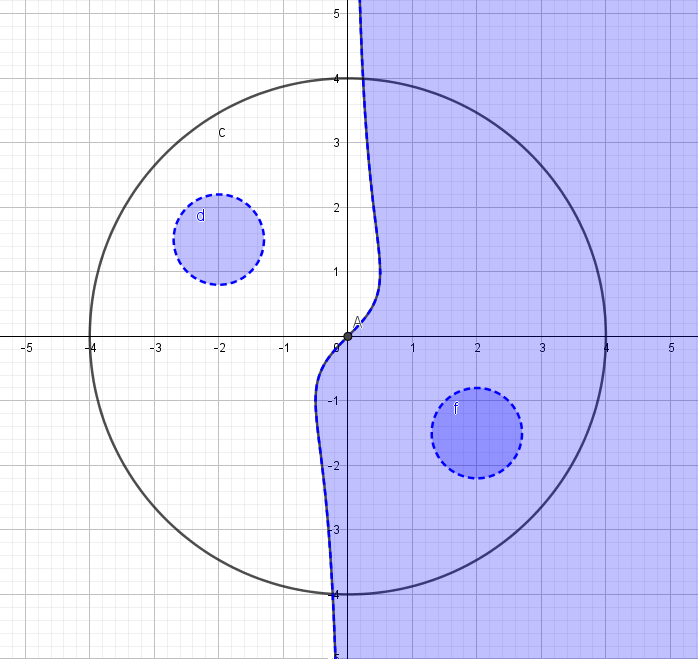
\includegraphics[width=\textwidth]{Tests/Test5/YYGG}
            \caption{Salida del software \texttt{GeoGebra}}
            \label{fig:YYGG}
        \end{subfigure}
        \caption{Ejemplo 5 - patrón yin-yang}
        \label{fig:YYInitialPlots}
\end{figure}
Una vez dibujadas las ecuaciones, se generó una base de datos de aproximadamente $n \approx \num{800}$ observaciones con una distribución uniforme dentro del círculo usando coordenadas polares. A estos puntos se les asignó la categoría cero, posteriormente se cambió la categoría a los puntos que cumplieran con las desigualdades. Después, se le añadió algo de ruido normal a cada punto para darle aleatoriedad a la base de datos pero manteniendo el patrón y finalmente, se escala la base para centrarla en cero.  

Se corrieron un sinfín de realizaciones del modelo, tratando de calibrar los parámetros $\MJK$ para captar de la mejor manera posible el patrón. Sin embargo y aunque el modelo casi siempre lograba una precisión de cerca de $85\%$, no se logra la clasificación esperada identificando los puntos de color dentro de las áreas opuestas. De cualquier forma se observa como el algoritmo está tratando de encontrar este patrón. En la figura \ref{fig:YY} se pueden ver fronteras de algunos de los mejores modelos.\footnote{En la imagen \ref{fig:YY3}, el modelo detecta relativamente bien la curva que separa las regiones y detecta de forma aislada el circulo azul de la esquina inferior derecha.}
\begin{figure}[htp]
        \centering
        \begin{subfigure}[b]{0.45\textwidth}
            \centering
            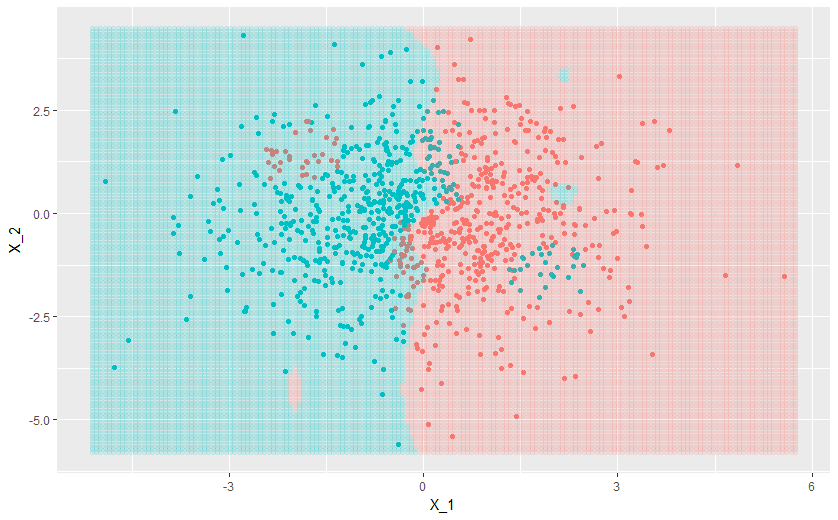
\includegraphics[width=\textwidth]{Tests/Test5/YY3}
            \caption{Sobre-ajuste}
			\label{fig:YY3}
        \end{subfigure}
        \hfill
        \begin{subfigure}[b]{0.45\textwidth}  
            \centering 
            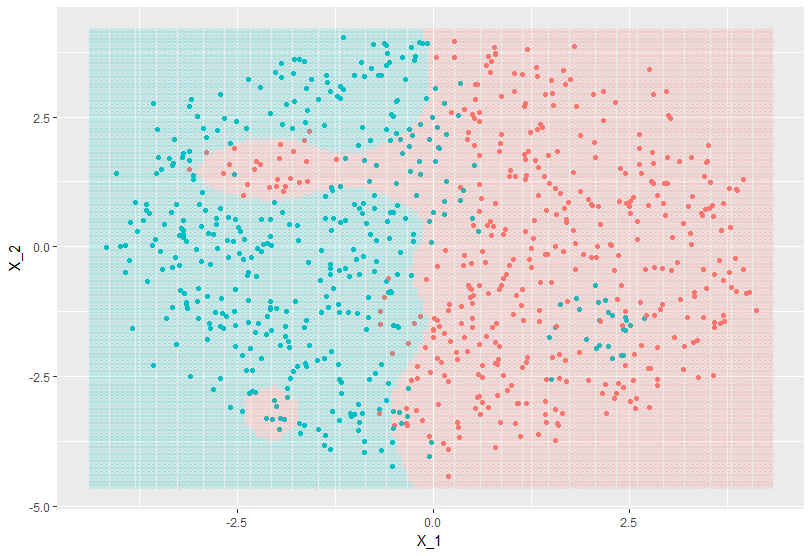
\includegraphics[width=\textwidth]{Tests/Test5/YY2}
            \caption{Mejor modelo}
			\label{fig:YY2}
        \end{subfigure}
        \vskip\baselineskip
        \begin{subfigure}[b]{0.45\textwidth}
            \centering
            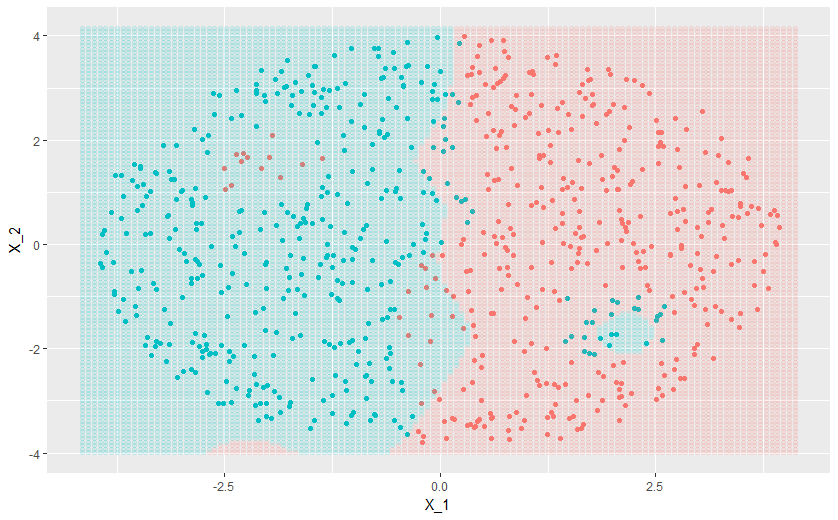
\includegraphics[width=\textwidth]{Tests/Test5/YY1}
			\caption{Falta de precisión}
			\label{fig:YY1}
        \end{subfigure}
        \hfill
        \begin{subfigure}[b]{0.45\textwidth}  
            \centering 
            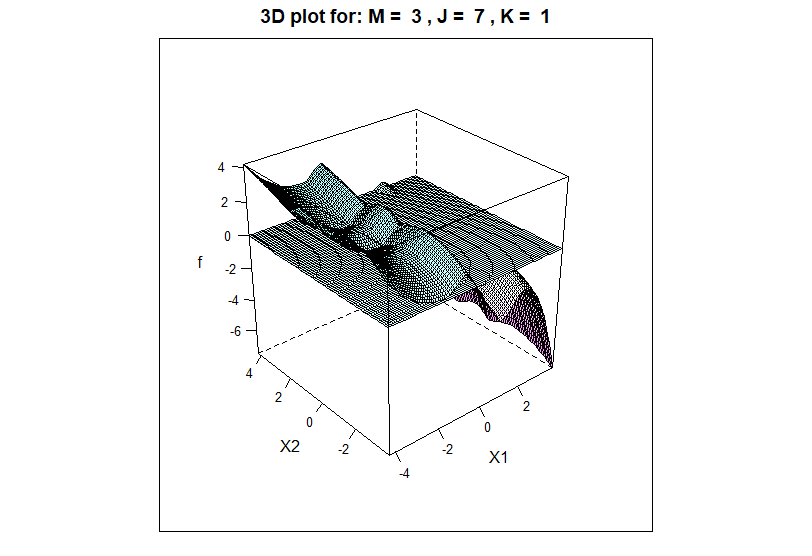
\includegraphics[width=\textwidth]{Tests/Test5/YY3D}
			\caption{Gráfico 3D para uno de los modelos}
			\label{fig:YY3D}
        \end{subfigure}
    	\caption{Fronteras de varios modelos para datos yin-yang}
        \label{fig:YY}
\end{figure}
Para las imágenes \ref{fig:YY1} y \ref{fig:YY2}, se observa como el modelo está tratando de encontrar las regiones anidadas, sin embargo, nunca se logra de forma precisa. Finalmente la imagen \ref{fig:YY3D}, muestra una, de las muchas representaciones 3D que se hicieron al tratar de ajustar esta base de datos. Precisamente en esta última imagen esconde el porqué no se logró hacer la estimación correcta: la dependencia implícita entre los nodos. Estos nodos, en realidad están dividiendo el espacio bi-dimensional en una malla cuadriculada donde las interacciones son difíciles de discernir. Conforme aumenta el número de nodos, más complejo se vuelve el modelo. Es por ello, que los picos y valles se repiten en un patrón uniforme. Asimismo, dada la naturaleza global de los polinomios y esta interacción, el modelo tiene esta estructura decreciente siempre, derivando que los picos y los valles nunca alcancen las regiones extremas en polos opuestos. De igual forma, la uniformidad y simetría impar, inherente a esta base de datos, llevó a que la estimación de los parámetros fuera óptima dentro de las capacidades del modelo. Otra desventaja de esta base, es que estos modelos se tuvieron que correr con un número grande de nodos $J \approx 20$, derivando en un número de parámetros aún mayor.

\section{Ejemplo 6 - el modelo en la práctica} \label{sec:T6}
Hasta ahora, todos los resultados de este trabajo han sido sobre bases de datos simuladas. Claramente  se forman imágenes atractivas por construcción, sin embargo, no se está prediciendo nada en realidad pues se utiliza una metodología \textit{dentro de muestra} para enfatizar las posibles fronteras del modelo. Por lo tanto y como último ejemplo, se presenta la base de datos de cáncer de mama de la Universidad de Wisconsin. Esta base de datos, es citada en varios trabajos de los años noventa, donde se tratan de hacer clasificaciones binarias usando una serie de procedimientos más robustos que los tradicionales GLM,  \citet{mangasarian1990pattern} y \citet{bennett1992robust}.

De manera general y sin entrar en el detalle biológico de las variables como tal, se presenta un análisis exploratorio preliminar que se lleva a cabo para seleccionar, de forma completamente subjetiva, las que se consideren relevantes.  La base de datos cuenta con $n = 699$ observaciones de las cuales el $34.5\%$ representan pacientes infectados con tumores malignos representados por el color rojo (etiqueta cero). Se cuenta con diez covariables (dimensiones) médicas sobre las características de los tumores como lo son: el tamaño, la uniformidad de la pared celular y la cromatina.\footnote{Forma en la que se presenta la cadena de ADN en el núcleo celular.} En la figura \ref{fig:BCExp}, se muestran los gráficos de puntos pareados para todas las posibles combinaciones de covariables además de cierta información adicional.
\begin{figure}[h]
	\centering
	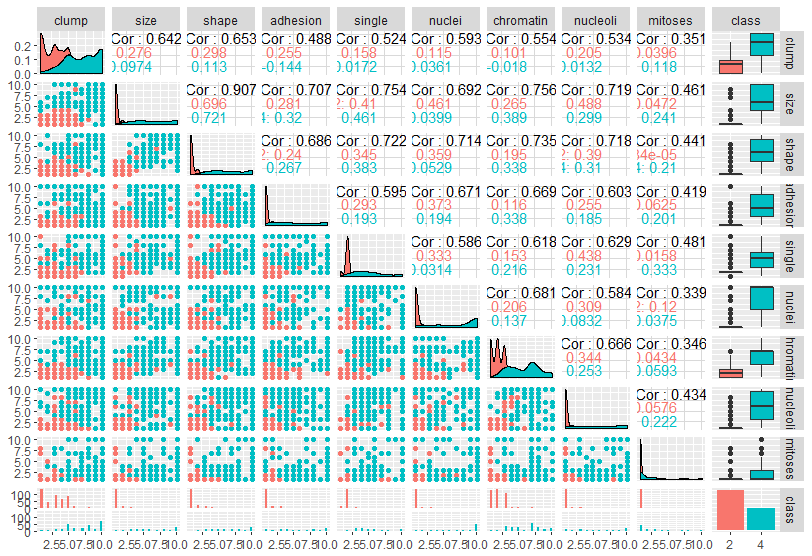
\includegraphics[width=.9\textwidth]{Tests/Test6/BCExp}
	\caption{Análisis exploratorio para selección de variables}
	\label{fig:BCExp}
\end{figure}
Se hace notar que las covariables están codificadas en una escala a 10 puntos, por lo tanto, la representación gráfica de los datos se ve más como una cuadrícula que como un espacio real de variables. Derivado de esta exploración previa, se seleccionan las covariables \textit{clump, size} y \textit{chromatin} debido a que parecieran ser las que mejor separan el espacio.\footnote{Estas covariables corresponden a el espesor de los tumores, su tamaño y la textura de la cromatina en las células respectivamente.} En la figura \ref{fig:BCJP} se presentan dos gráficos de puntos con algo de ruido para hacer notar que las regiones son un poco más complejas de lo que podría parecer en una primera exploración, además se tienen puntos idénticos con clasificaciones contrarias. Sin embargo, a simple vista se detecta cierto patrón en los datos.
\begin{figure}[h]
        \centering
        \begin{subfigure}[b]{0.45\textwidth}
            \centering
            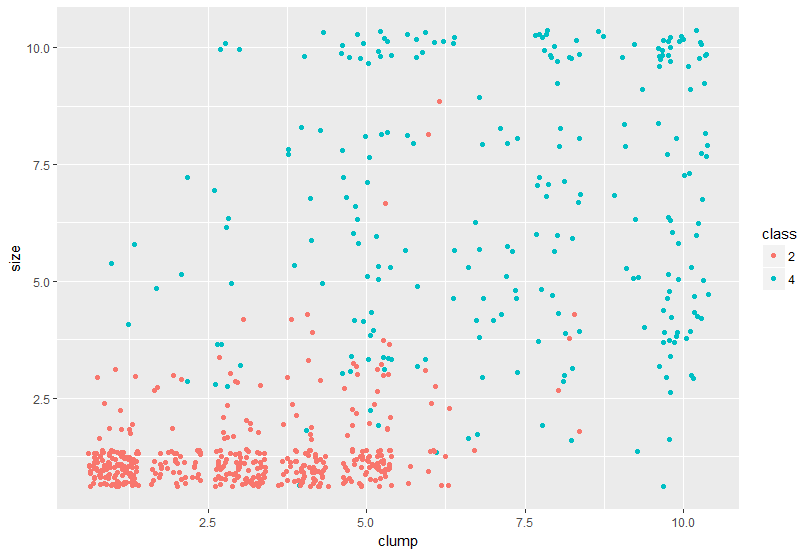
\includegraphics[width=\textwidth]{Tests/Test6/BCJP1}
            \caption{Variables \textit{clump} y \textit{chromatin}}
			\label{fig:BCJP1}
        \end{subfigure}
        \hfill
        \begin{subfigure}[b]{0.45\textwidth}  
            \centering 
            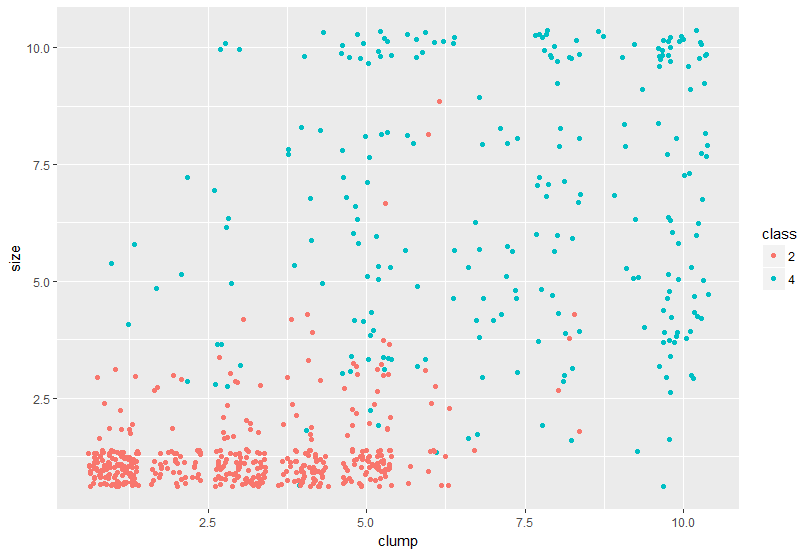
\includegraphics[width=\textwidth]{Tests/Test6/BCJP1}
            \caption{Variables \textit{clump} y \textit{size}}
			\label{fig:BCJP2}
        \end{subfigure}
		\caption{Gráficos de puntos con ruido para separar las observaciones}
		\label{fig:BCJP}
\end{figure}

Para poder hablar de predicción como tal, tiene que existir una base de datos contra la cual probar las estimaciones del modelo. Por lo tanto, la base original se parte en dos: un conjunto de entrenamiento con el $60\%$ de las observaciones ($n_{\text{train}} = 409$) y un conjunto de prueba con las observaciones restantes ($n_{\text{test}} = 274$) sobre las que se evaluará el modelo.\footnote{La diferencia de 16 observaciones entre la suma de entrenamiento y prueba, contra las 699 originales, se debe a que estas estaban incompletas y por lo tanto se descartan.} La realización final de entrenamiento del modelo se resume en la tabla \ref{ej:BC}, se escogen segmentos de recta continuos sobre tres nodos. Los resultados numéricos sobre la base de datos de prueba se presentan en la tabla \ref{tab:BCRes} y el análisis de convergencia a través de las medias ergódicas en la figura \ref{fig:T6ME}. Asimismo, se presenta cada $\hat{f}_j\quad j = 1,2,3$ en las figuras \ref{fig:T6F1}, \ref{fig:T6F2} y \ref{fig:T6F3} respectivamente.

Haciendo una predicción fuera de muestra los resultados son buenos logrando una precisión del $95.6\%$. Asimismo, se resalta que inclusive en dimensiones ($d = 3$) más altas si se escogen los parámetros adecuados $\MJK$, el número total de parámetros ($\lambda = 13$) no necesita aumentar demasiado para lograr una buena separación del espacio.\footnote{Se corrieron otras realizaciones del modelo aumentando el número de covariables $d$ y ajustando los parámetros $\MJK$. Sin embargo, no logró aumentar significativamente la precisión del modelo.} Sin embargo, derivado también del número de covariables es que no se pueden hacer una visualización en el plano cartesiano $\mathbb{R}^2$ como en los ejemplos anteriores. No obstante, la convergencia es clara y los resultados buenos, incluso usando segmentos de recta y un número de nodos pequeño. Se hace notar que la codificación de las covariables usando una escala de diez puntos no es óptima para un modelo que se construye pensando en un espacio real de covaraibles $\mathcal{X}^d$, sin embargo, no parece afectar la estimación de los parámetros. 

\begin{table}[ht]
$$\paramsmod{2}{4}{1}{4}{13}{409}{\num{50000}}{\num{10000}}{0}$$
\caption{Ejemplo 6 - datos médicos de cáncer}
\label{ej:BC}
\end{table}

\begin{table}[ht]
\begin{align*}
\resultados{\text{Media posterior}}{95.6}{0.1561}
\qquad\qquad\qquad
\matconf{169}{9}{178}{3}{93}{96}{172}{102}{274}
\end{align*}
\caption{Ejemplo 6 - resultados}
\label{tab:BCRes}

\end{table}
\begin{figure}[ph]
        \centering
        \begin{subfigure}[b]{0.45\textwidth}
            \centering
            \includegraphics[width=\textwidth]{Tests/Test6/T6ME}
            \caption{Medias ergódica}
			\label{fig:T6ME}
        \end{subfigure}
        \hfill
        \begin{subfigure}[b]{0.45\textwidth}  
            \centering 
            \includegraphics[width=\textwidth]{Tests/Test6/T6F1}
            \caption{$\hat{f}_1(x_1)$ con ruido}
			\label{fig:T6F1}
        \end{subfigure}
        \vskip\baselineskip
        \begin{subfigure}[b]{0.45\textwidth}
            \centering
            \includegraphics[width=\textwidth]{Tests/Test6/T6F2}
			\caption{$\hat{f}_2(x_2)$ con ruido}
			\label{fig:T6F2}
        \end{subfigure}
        \hfill
        \begin{subfigure}[b]{0.45\textwidth}  
            \centering 
            \includegraphics[width=\textwidth]{Tests/Test6/T6F3}
			\caption{$\hat{f}_3(x_3)$ con ruido}
			\label{fig:T6F3}
        \end{subfigure}
    	\caption{Media ergódica y funciones $\hat{f}_j(x_j)\quad j=1,2,3$}
        \label{fig:T6Plots}
\end{figure}
\end{document}
